\section{Durchführung}
\label{sec:Durchfuehrung}
Für die Bestimmung der Leerlaufspannung und der Innenwiderstände wird ein hochohmiges Spannungsmessgerät benutzt, sodass der Spannungsverlust und damit Messunsicherheiten durch das Messgerät klein sind.
Der Innenwiderstand des Messgerätes beträgt $\SI{10}{\mega\ohm}$.
Zur Bestimmung der Leerlaufspannung und des Innenwiderstandes werden zwei verschiedene Spannungsquellen benutzt.

\subsection{Messung an einer Monozelle}
\label{sec:drchf_monozelle}
Die Leerlaufspannung wird mit einem Voltmeter bestimmt.\
Hierzu wird zwischen Spannungsquelle und Messgerät kein Verbraucher geschaltet.
\begin{figure}
	\centering
	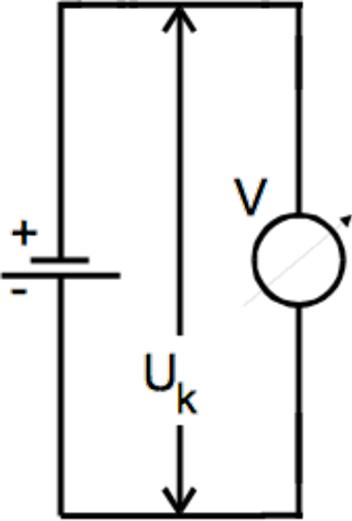
\includegraphics[width=3cm]{Bilder/Leerlauf.pdf}
	\caption{Schaltung zur Messung der Leerlaufspannung.\cite{V301}}
	\label{fig:leerlauf}
\end{figure}

Anschließend wird die Spannung an den Klemmen $U_\text{k}$ sowie der Strom $I$ durch einen Verbraucher variablen Widerstandes $R$ mit Volt- bzw. Amperemetern gemessen.
Die Schaltung wird in Abbildung \ref{fig:ri} gezeigt.
Nach Schließen des Stromkreises werden die Werte von den Messgeräten abgelesen, der Widerstand $R$ variiert und die Messung wiederholt, sodass insgesamt 10 Messwertpaare aufgenommen werden.
Der Widerstand ist von 0-50\,\si{\ohm} zu wählen.
Die Schaltung wird im Weiteren durch eine weitere, ideale Spannungsquelle erweitert.
Diese wird gemäß Schaltskizze \ref{fig:rimgu} so eingebaut, dass der Strom in umgekehrter Richtung als in Schaltung \ref{fig:ri} fließt.
Analog werden nach Einschwingen der Messgeräte die Klemmenspannung $U_\text{k}$ und der Strom $I$ aufgenommen, der Widerstand $R$ variiert und der Vorgang widerholt, bis 10 Messwertpaare aufgenommen werden.
\begin{figure}
	\begin{subfigure}{0.5\textwidth}
	\centering
	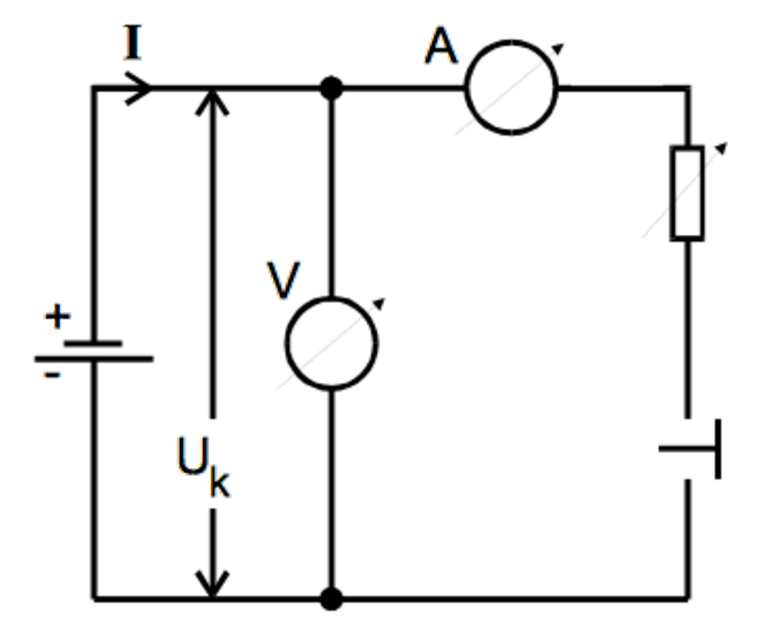
\includegraphics[width=0.8\textwidth]{Bilder/Messung1.pdf}
	\caption{Schaltung ohne Gegenspannungsmethode.}
	\label{fig:ri}
	\end{subfigure}
	\begin{subfigure}{0.5\textwidth}
	\centering
	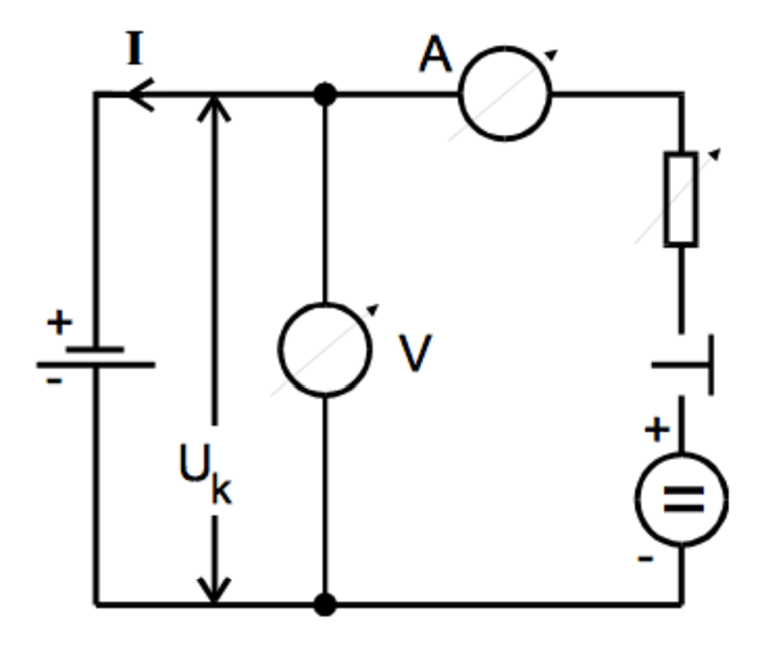
\includegraphics[width=0.8\textwidth]{Bilder/Messung2.pdf}
	\caption{Schaltung mit Gegenspannungsmethode.}
	\label{fig:rimgu}
	\end{subfigure}
	\caption{Schaltung zur Messung des Innenwiderstandes.\cite{V301}}
\end{figure}

\subsection{Messung an einem Funktionsgenerator}
\label{sec:drchf_funktion}
Ähnlich zu \ref{sec:drchf_monozelle} wird die Spannungsquelle mit einem ohmschen Verbraucher verbunden, wobei parallel zur Spannungsquelle ein Voltmeter und in Reihe zum Verbraucher ein Amperemeter geschaltet wird.
Die Aufbauskizze ist \ref{fig:ri} ähnlich.
Für die erste Messung wird der Funktionsgenerator auf Sinusschwingung eingestellt, der Widerstand ist von 0,5-5\,\si{\kilo\ohm} zu wählen.
Analog zu \ref{sec:drchf_monozelle} werden die Klemmenspannung  $U_\text{k}$ und der Strom $I$ aufgenommen, der Widerstand $R$ variiert und der Vorgang widerholt, bis 10 Messwertpaare aufgenommen werden.
Der Funktionsgenerator wird auf Rechteckspannung umgestellt und das Verfahren wiederholt, wobei
der Widerstand von 50-250\,\si{\ohm} gewählt wird.
